\documentclass{article}
\usepackage{aligned-overset}
\usepackage{amsmath}
\usepackage{amssymb}
\usepackage{bm}
\usepackage[shortlabels]{enumitem}
\usepackage{hyperref}
\usepackage[utf8]{inputenc}
\usepackage{pdflscape}
\usepackage{mathtools}
\usepackage{physics}
\usepackage{tabularx}
\usepackage{titling}
\usepackage{fancyhdr}
\usepackage{xfrac}
\usepackage{pgfplots}

\pgfplotsset{compat = newest}
\usetikzlibrary{intersections}
\usepgfplotslibrary{fillbetween}


\author{}
\date{SoSe 2021}
\title{Hausaufgabe 02 Analysis - Weiterführende Konzepte}

\pagestyle{fancy}
\fancyhf{}
\lhead{\thetitle}
\rhead{\theauthor}
\lfoot{\thedate}
\rfoot{Seite \thepage}

\begin{document}

\section*{Hausaufgabe 1}

Untersuchen Sie, ob die folgenden Aussagen wahr oder falsch sind.
Begründen Sie Ihre Antworten.

\begin{enumerate}[(i)]
\item Die Funktion $F(x) \coloneqq x\abs{x}, x \in [-1,1]$, ist die Stammfunktion einer
  Funktion $f \in R([-1, 1])$.

  \label{dia:1.1}
  \begin{tikzpicture}
    \begin{axis}[
        axis lines=middle,
        xmax = 1.2,
        xmin = -1.2,
        ymax = 1.2,
        ymin = -1.2,]
      \addplot [
        domain=-1:1,
        name path=f,
        samples=100,
        very thick, blue]{x * abs(x)};
    \end{axis}
  \end{tikzpicture}

  $F(x) = \begin{cases}
    x^2 & x \geq 0 \\
    - x^2 & x < 0 \\
  \end{cases}, F'(x) = \begin{cases}
    2x & x \geq 0 \\
    -2x & x < 0 \\
  \end{cases} = 2 \abs{x} = f(x)$.
  Die Funktion $f(x)$ ist auf dem kompakten Intervall $[-1, 1]$ stetig, somit ist
  $f \in R([-1, 1])$ und die Aussage ist wahr.
  
\item Die Funktion $f(x) \coloneqq \text{sign}(x) \sqrt{\abs{x}}, x \in [-1,1]$, besitzt
  auf $[-1,1]$ eine Stammfunktion.

  \label{dia:1.2}
  \begin{tikzpicture}
    \begin{axis}[
      axis lines=middle,
      xmax = 1.2,
      xmin = -1.2,
      ymax = 1.2,
      ymin = -1.2,]
      \addplot [
        domain=-1:1,
        name path=f,
        samples=100,
        very thick, blue]{sign(x) * sqrt(abs(x))};
    \end{axis}
  \end{tikzpicture}

  Die Funktion ist auf den Intervallen $[-1, 0)$ und $(0, 1]$ stetig.
  Weiterhin ist $\lim_{x \to 0-} f(x) = \lim_{x \to 0+} f(x) = f(x) = 0$.
  Somit ist die Funktion auf dem kompakten Intervall $[-1, 1]$ stetig und
  besitzt auf diesem Intervall eine Stammfunktion.
  Damit ist die Aussage wahr.

\newpage
\item Die Funktion $f(x) \coloneqq \text{sign}(x) \sqrt{\abs{x + \frac{1}{2}}}, x \in [-1,1]$, besitzt
  auf $[-1,1]$ eine Stammfunktion.

  \label{dia:1.2}
  \begin{tikzpicture}
    \begin{axis}[
        axis lines=middle,
        xmax = 1.2,
        xmin = -1.2,
        ymax = 1.2,
        ymin = -1.2,]
      \addplot [
        domain=-1:-0.01,
        name path=f,
        samples=100,
        very thick, blue]{sign(x) * sqrt(abs(x + 0.5))};
      \node [
        circle,
        fill,
        inner sep=1pt, blue] at (0,0) {};
      \addplot [
        domain=0.01:1,
        name path=f,
        samples=100,
        very thick, blue]{sign(x) * sqrt(abs(x + 0.5))};
    \end{axis}
  \end{tikzpicture}

  $\lim_{x \to 0-} f(x) = - \sqrt{\frac{1}{2}}, \lim_{x \to 0+} f(x) = \sqrt{\frac{1}{2}}$ und $f(0) = 0$.
  Damit besitzt die Funktion an der Stelle $0$ einen Sprung.
  Aus dem Satz von Darboux folgt, dass die Funktion auf dem Intervall $[-1, 1]$ keine Stammfunktion besitzt.
\end{enumerate}

\section*{Hausaufgabe 2}

Ermitteln Sie größtmögliche Intervalle $I \in \mathbb{R}$ auf denen die folgenden Ausdrücke
$f(x)$ Stammfunktionen besitzen.
Berechnen Sie zughörige Stammfunktionen $F \colon I \to \mathbb{R}$
durch Anwendung des Hauptsatzes.

\begin{enumerate}[a)]
\item $f(x) = \frac{\sin x}{\sqrt{9 + \cos x}}$

  $\mathbb{D}_f = \mathbb{R}$
  \begin{flalign*}
    u &= 9 + \cos x & \\
    du &= - \sin(x) \,dx & \\
    dx &= - \frac{1}{\sin x} \,du &
  \end{flalign*}
  \begin{flalign*}
    F(x) &= \int \frac{\sin x}{\sqrt{9 + \cos x}} \, dx = \int \frac{\sin x}{\sqrt{9 + \cos x}} \cdot \left( - \frac{1}{\sin x} \right) \,du & \\
    \overset{\substack{\text{Substitution} \\ u = 9 + \cos x}}&= - \int \frac{1}{\sqrt{u}} \,du =  - \int u^{\frac{1}{2}} \,du & \\
         &= -2 u^{\frac{1}{2}} = -2 \sqrt{u} & \\
    F(x) &= -2 \cdot \sqrt{9 + \cos x}, x \in \mathbb{R} & 
  \end{flalign*}
  
\item $f(x) = \frac{\sin x}{\cos^2 x}$

  $(a_n)_{n \in \mathbb{Z}} \coloneqq \pi n - \frac{\pi}{2}, \mathbb{D}_f = \mathbb{R} \setminus (a_n)$
  \begin{flalign*}
    u &= \cos x & \\
    du &= - \sin(x) \,dx & \\
    dx &= - \frac{1}{\sin x} \,du &
  \end{flalign*}
  \begin{flalign*}
    F(x) &= \int \frac{\sin x}{\cos^2 x}\,dx = \int \frac{\sin x}{\cos^2 x} \cdot \left(- \frac{1}{\sin x} \right) \,du& \\
    \overset{\substack{\text{Substitution} \\ u = \cos x}}&= - \int \frac{1}{u^2} \,du = - \int u^{-2} \,du & \\
         &= - \left( - \frac{1}{u} \right) \\
    F(x) &= \frac{1}{\cos x}, x \in \mathbb{R} \setminus (a_n) 
  \end{flalign*}
\item $f(x) = \frac{4x \arctan(x^2)}{1 + x^4}$
    $\mathbb{D}_f = \mathbb{R}$
  \begin{flalign*}
    u &= \arctan(x^2) & \\
    du &= 2x \cdot \frac{1}{1 + \left( x^2 \right)^2} \,dx = \frac{2x}{1 + x^4} \,dx & \\
    dx &= \frac{1 + x^4}{2x} \,du &
  \end{flalign*}
  \begin{flalign*}
    F(x) &= \int \frac{4x \arctan(x^2)}{1 + x^4} \,dx = \int \frac{4x \arctan(x^2)}{1 + x^4} \cdot \frac{1 + x^4}{2x} \,du & \\
         &= \int 2 \arctan(x^2) \,du & \\
    \overset{\substack{\text{Substitution} \\ u = \arctan(x^2)}}&= \int 2 \cdot u \,du = 2 \int u \,du & \\
    F(x) &= u^2 = arctan^2\left( x^2 \right), x \in \mathbb{R}     
  \end{flalign*}
\end{enumerate}

\newpage
\section*{Hausaufgabe 3}

Ermitteln Sie größtmögliche Intervalle $I \in \mathbb{R}$ auf denen
die folgenden Ausdrücke $f(x)$ Stammfunktionen besitzen.
Berechnen Sie zughörige Stammfenktionen $F: I \to \mathbb{R}$ durch
Anwendung des Hauptsatzes. \\
\textbf{Hinweis:} Substitutionsmethode oder partielle Integration anwenden!

\begin{enumerate}[(i)]
\item Ermitteln Sie Stammfunktionen der folgenden Ausdrücke $f(x)$ auf größtmöglichen
  Intervallen $I \in \mathbb{R}$
  \begin{enumerate}[a)]
  \item $f(x) \coloneqq x \exp(3x)$

    \label{dia:3.1.a}
    \begin{tikzpicture}
      \begin{axis}[
          axis lines=middle,
          xmax = 1.1,
          xmin = -1.1,
          ymax = 9,
          ymin = -0.8]
        \addplot [
          domain=-2:2,
          name path=f,
          samples=100,
          very thick, blue]{x * exp(3 * x)};
      \end{axis}
    \end{tikzpicture}

    $\mathbb{D}_f = \mathbb{R}$

    $u'(x) = \exp(3x), u(x) = \frac{1}{3} \exp(3x), v(x) = x l, v'(x) = 1$
    \begin{align*}
      \int f(x)\,dx &= u(x) \cdot v(x) - \int v'(x) \cdot u(x) \,dx \\
                    &= \frac{1}{3} \exp(3x) \cdot x  - \int 1 \cdot \frac{1}{3}\exp(3x) \,dx \\
                    &= \frac{1}{3} \exp(3x) \cdot x  - \frac{1}{3} \int \exp(3x) \,dx \\
                    &= \frac{1}{3} \exp(3x) \cdot x  - \frac{1}{9} \exp(3x) \\
                    &= \frac{1}{9} \cdot 3 \cdot \exp(3x) \cdot x  - \frac{1}{9} \exp(3x) \\
      F(x) &= \frac{1}{9} \exp(3x) (3x - 1), x \in \mathbb{R}
    \end{align*}

  \newpage
  \begin{landscape}
    \item $f(x) \coloneqq \cos(\ln x) + \sin(\ln x)$
      \begin{flalign*}
        & \makebox[\textwidth]{} & %% This little hack ensures, that the whole width is used.
      \end{flalign*}

      \label{dia:3.1.b}
      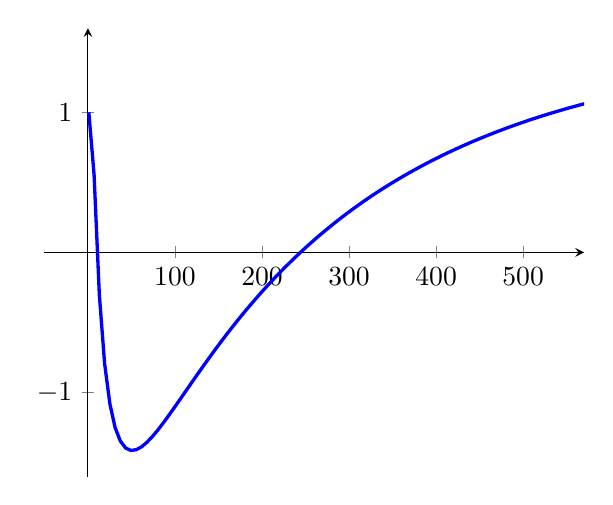
\begin{tikzpicture}
        \begin{axis}[
            axis lines=middle,
            xmax = 570,
            xmin = -50,
            ymax = 1.6,
            ymin = -1.6,]
          \addplot [
            domain=1:600,
            name path=f,
            samples=100,
            very thick, blue]{cos(deg(ln(x))) + sin(deg(ln(x)))};
        \end{axis}
      \end{tikzpicture}

      $\mathbb{D}_f = \mathbb{R}_{>0}$

      Zuerst wird die Funktion aufgeteilt in $g(x) = \cos(\ln(x))$ und $h(x) = \sin(\ln(x))$.
      Damit lässt sich $f(x) = \cos(\ln(x)) + \sin(\ln(x))$ als $f(x) = g(x) + h(x)$ schreiben.
      Das unbestimmte Integral $\int f(x)\,dx$ wird nun zu der Summe $\int g(x)dx + \int h(x)dx$.

      \newpage
      \begin{enumerate}[b) (i)]
        \item \textbf{Integration von $g(x) = \cos(\ln(x))$ per Substitution}
          \begin{flalign*}
            u &= \ln(x) \iff e^u = e^{\ln(x)} = x & \\
            du &= \frac{1}{x}dx & \\
            dx &= x \cdot du = e^u \cdot du
          \end{flalign*}
          \begin{flalign*}
            G(x) &= \int \cos(\ln(x))dx \overset{\substack{\text{Substitution} \\ u = \ln(x)}}= \int \cos(u) e^udu &
          \end{flalign*}
          \begin{flalign*}
            \int \cos(u) e^udu \overset{\substack{\text{Partielle}\\\text{Integration}}}
                                &= e^u \cos(u) -\underset{\makebox[0pt]{$\displaystyle \left(e^u (-\sin(u)) - \int e^u (-\cos(u))du\right)$}}
                                  {\underbrace{\int e^u (-\sin(u))du}} &\\
                                &= e^u \cos(u) - \left(e^u (-\sin(u)) + \int e^u \cos(u)du\right) &\\
                                &= e^u \cos(u) + e^u \sin(u) - \int e^u \cos(u)du && | + \int e^u \cos(u)du &\\
            2 \int \cos(u) e^udu &= e^u \cos(u) + e^u \sin(u) && | :2 &\\
                                &= \frac{e^u \cos(u) + e^u \sin(u)}{2} &\\
            \overset{\text{Substituiere } u = \ln(x)}&=  \frac{e^{\ln(x)} \cos(\ln(x)) + e^{\ln(x)} \sin(\ln(x))}{2} &\\
            G(x) &= \frac{x (\cos(\ln(x)) + \sin(\ln(x)))}{2}
          \end{flalign*}
        \newpage 
        \item \textbf{Integration von $h(x) = \sin(\ln(x))$ per Substitution}
          \begin{flalign*}
            u &= \ln(x) \iff e^u = e^{\ln(x)} = x & \\
            du &= \frac{1}{x}dx & \\
            dx &= x \cdot du = e^u \cdot du
          \end{flalign*}
          \begin{flalign*}
            H(x) &= \int \sin(\ln(x))dx \overset{\substack{\text{Substitution} \\ u = \ln(x)}}= \int \sin(u) e^udu &
          \end{flalign*}
          \begin{flalign*}
            \int \sin(u) e^udu \overset{\substack{\text{Partielle}\\\text{Integration}}}
                                &= e^u \sin(u) -\underset{\makebox[0pt]{$\displaystyle \left(e^u \cos(u) - \int e^u (-\sin(u))du\right)$}}
                                  {\underbrace{\int e^u \cos(u)du}} &\\
                                &= e^u \sin(u) - \left(e^u \cos(u) - \int e^u (-\sin(u))du\right) &\\
                                &= e^u \sin(u) - e^u \cos(u) - \int e^u \sin(u)du && | + \int e^u \sin(u)du &\\
            2 \int \sin(u) e^udu &= e^u \sin(u) - e^u \cos(u) && | :2 &\\
                                &= \frac{e^u \sin(u) - e^u \cos(u)}{2} &\\
            \overset{\text{Substituiere } u = \ln(x)}&=  \frac{e^{\ln(x)} \sin(\ln(x)) - e^{\ln(x)} \cos(\ln(x))}{2} &\\
            H(x) &= \frac{x (\sin(\ln(x)) - \cos(\ln(x)))}{2}
          \end{flalign*}
      \end{enumerate}

      \begin{flalign*}
        F(x) &= G(x) + H(x) &\\
             &= \frac{x (\cos(\ln(x)) + \sin(\ln(x)))}{2} + \frac{x (\sin(\ln(x)) - \cos(\ln(x)))}{2} &\\
             &= x \cdot \frac{\cos(\ln(x)) + \sin(\ln(x)) + \sin(\ln(x)) - \cos(\ln(x))}{2} &\\
             &= x \cdot \sin(\ln(x)), x \in \mathbb{R}_{>0}
      \end{flalign*}
      \begin{flalign*}
        & \makebox[\textwidth]{} & %% This little hack ensures, that the whole width is used.
      \end{flalign*}
    \item $f(x) \coloneqq \frac{\ln x}{x^3}$

      $\mathbb{D} = \mathbb{R}_{>0}$

      $u'(x) = x^{-3}, u(x) = -\frac{1}{2}x^{-2}, v(x) = \ln(x), v'(x) = \frac{1}{x}$
      \begin{align*}
        \int f(x)\,dx &= u(x) \cdot v(x) - \int v'(x) \cdot u(x) \,dx \\
                      &= -\frac{1}{2} x^{-2} \cdot \ln(x) - \int \frac{1}{x} \cdot \left(-\frac{1}{2} x^{-2}\right) \,dx \\
                      &= -\frac{1}{2} x^{-2} \cdot \ln(x) - \int -\frac{1}{2} x^{-3} \,dx \\
                      &= -\frac{1}{2} x^{-2} \cdot \ln(x) - \frac{1}{4} x^{-2} \,dx \\
        F(x) &= -\frac{1}{2} x^{-2} (ln(x) + \frac{1}{2}), x \in \mathbb{R}_{>0}
      \end{align*}
    \end{landscape}
  \end{enumerate}

\newpage
\item Stellen Sie für die folgenden Integrale
  \[
    F_v(x) \coloneqq \int_1^x t \ln^n(t) \,dt, x \in (0, \infty)
  \]
  eine Rekursionsformel bzgl. $n \in \mathbb{N}$ auf.
  Geben Sie explizite Darstellungen von $F_0, F_1, F_2$ an.

  \begin{flalign*}
    n = 0: F_0(x) &= \int_1^x t \ln^0(t) \,dt, x \in (0, \infty) &\\
                  &= \int_1^x t \cdot 1 \,dt, x \in (0, \infty) = \left[ \frac{1}{2}x^2 \right]_0^x
                    = \frac{1}{2}x^2 &\\
    n \geq 1: F_n(x) &= \int_1^x t \ln^n(t) \,dt, x \in (0, \infty) &\\
                     &= \frac{1}{2}t^2 \cdot \ln^n(t) {\Big |}_0^x - \frac{1}{2} \int_0^x t^2 \cdot
                       \colorbox{yellow}{$\displaystyle n\frac{\ln^{n-1}(t)}{t}$} \,dt, x \in (0, \infty) \\
                     &= \frac{1}{2} \left( x^2 \cdot \ln^n(x) - n \cdot
                       \underset{= F_{n - 1}(x)}{
                         \underbrace{\int_0^x t \cdot \ln^{n-1}(t) \,dt}} \right), x \in (0, \infty) \\
    F_1(x) &= \frac{1}{2} x^2 \left( \ln(x) - \frac{1}{2} \right) & \\
    F_2(x) &= \frac{1}{2} x^2 \left( \ln^2(x) - \ln(x) + \frac{1}{2} \right) & \\
  \end{flalign*}

  \colorbox{yellow}{Ableitung von $f(x) = \ln^n(x)$:}

  $g(x) = x^n, g'(x) = n \cdot x^{n - 1}, h(x) = \ln(x), h'(x) = \frac{1}{x}$

  $f(x) = g(h(x)), f'(x) = g'(h(x)) \cdot h'(x) = n \cdot \ln^{n-1}(x) \cdot \frac{1}{x} = n \frac{\ln^{n-1}(x)}{x}$
\end{enumerate}

\newpage
\section*{Hausaufgabe 4}

Die Funktionen $f, g \colon \mathbb{R} \to \mathbb{R}$ definiert durch
$f(x) = x^3 - 2x^2 + x$ und $g(x) = \frac{1}{2}x^2$ umschließen im 1.
Quadranten einen beschränkten Berebich $B$.
Skizzieren Sie diesen Bereich $B$ und berechnen Sie dessen Flächeninhalt.
\\

\label{dia:4}
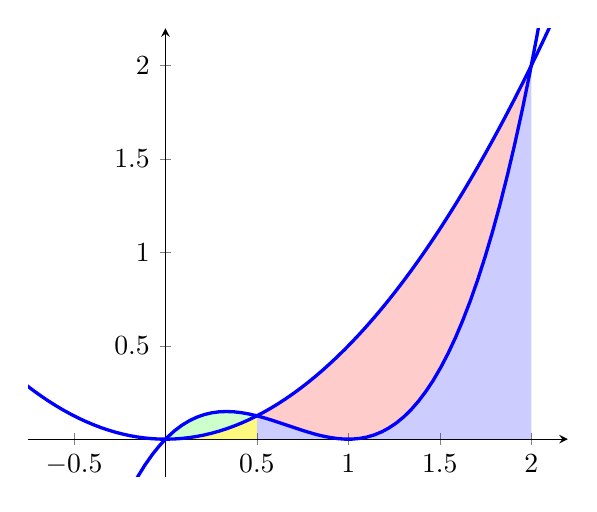
\begin{tikzpicture}
  \begin{axis}[
      axis lines=middle,
      xmax = 2.2,
      xmin = -0.75,
      ymax = 2.2,
      ymin = -0.2,]
    \addplot [
      domain=-1:3,
      name path=f,
      samples=100,
      very thick, blue]{x^3 - 2*x^2 + x};
    \path[name path=axisa] (axis cs:0,0) -- (axis cs:0.5,0);
    \path[name path=axisb] (axis cs:0.5,0) -- (axis cs:2,0);
    \addplot [
      thick,
      color=blue,
      fill=blue, 
      fill opacity=0.2
    ]
    fill between[
      of=f and axisb,
      soft clip={domain=0.5:2},
    ];
    \addplot [
      domain=-1:3,
      name path=g,
      samples=100,
      very thick, blue]{0.5 * x^2};
    \addplot [
      thick,
      color=yellow,
      fill=yellow, 
      fill opacity=0.5
    ]
    fill between[
      of=g and axisa,
      soft clip={domain=0:0.5},
    ];
    \addplot [
      thick,
      color=green,
      fill=green, 
      fill opacity=0.2
    ]
    fill between[
      of=f and g,
      soft clip={domain=0:0.5},
    ];
    \addplot [
      thick,
      color=red,
      fill=red, 
      fill opacity=0.2
    ]
    fill between[
      of=f and g,
      soft clip={domain=0.5:2},
    ];  
  \end{axis}
\end{tikzpicture}

\textbf{Schnittstellen der beiden Funktionen berechnen}:
\begin{align*}
  f(x) &= g(x) \\
  x^3 - 2x^2 + x &= \frac{1}{2}x^2 && | :x \text{ $x_1 = 0$ ist eine Lösung} \\
  x^2 - 2x + 1 &= \frac{1}{2}x && | \cdot 2 \\
  2 x^2 - 4x + 2 &= x && | - x \\
  2 x^2 - 5x + 2 &= 0 \\
\end{align*}

\begin{align*}
  x_{2|3} &= \frac{5 \pm \sqrt{5^2 - 4 \cdot 2 \cdot 2}}{2 \cdot 2} \\
          &= \frac{5 \pm \sqrt{9}}{4} \\
  x_2 &= 0.5, \, x_3 = 2 
\end{align*}

\textbf{Stammfunktionen von $g$ und $f$ ermitteln}
\begin{align*}
  F(x) &= \frac{1}{4}x^4 - \frac{2}{3}x^3 + \frac{1}{2}x^2 \\
  G(x) &= \frac{1}{6}x^3 
\end{align*}

\newpage
\textbf{Fläche B berechnen}:

Die Fläche B setzt sich aus zwei Teilflächen - im \hyperref[dia:4]{Diagramm}
grün und rot markiert - zusammen.
Der Inhalt der grünen Teilfläche ($B_1$) errechnet sich aus
$B_1 = \int_{x_1}^{x_2} f(x) dx - \int_{x_1}^{x_2} g(x) dx$ und der Inhalt der roten
Teilfläche ($B_2$) aus
$B_2 = \int_{x_2}^{x_3} g(x) dx - \int_{x_2}^{x_3} f(x) dx$
\begin{align*}
  B_1 &= \left( F(x_2) - F(x_1) \right) - \left( G(x_2) - G(x_1) \right) \\
      &= F(x_2) - F(x_1) - G(x_2) + G(x_1) \\
      &= \sfrac{1}{4}(x_2)^4 - \sfrac{2}{3}(x_2)^3 + \sfrac{1}{2}(x_2)^2 - \sfrac{1}{4}(x_1)^4 + \sfrac{2}{3}(x_1)^3 - \sfrac{1}{2}(x_1)^2 -
        \sfrac{1}{6}(x_2)^3 + \sfrac{1}{6}(x_1)^3 \\
      &= \sfrac{1}{4}(x_2)^4 - \sfrac{5}{6}(x_2)^3 + \sfrac{1}{2}(x_2)^2 - \sfrac{1}{4}(x_1)^4 + \sfrac{5}{6}(x_1)^3 - \sfrac{1}{2}(x_1)^2 \\
      &= \sfrac{1}{4}\left(\sfrac{1}{2}\right)^4 - \sfrac{5}{6}\left(\sfrac{1}{2}\right)^3 + \sfrac{1}{2}\left(\sfrac{1}{2}\right)^2 -
        \sfrac{1}{4}(0)^4 + \sfrac{5}{6}(0)^3 - \sfrac{1}{2}(0)^2 \\
      &= \frac{7}{192}
\end{align*}
\begin{align*}
  B_2 &=\left( G(x_3) - G(x_2) \right) - \left( F(x_3) - F(x_2) \right) \\
      &= G(x_3) - G(x_2) - F(x_3) + F(x_2) \\
      &= \sfrac{1}{6}(x_3)^3 - \sfrac{1}{6}(x_2)^3 - \sfrac{1}{4}(x_3)^4 + \sfrac{2}{3}(x_3)^3 - \sfrac{1}{2}(x_3)^2 +
        \sfrac{1}{4}(x_2)^4 - \sfrac{2}{3}(x_2)^3 + \sfrac{1}{2}(x_2)^2 \\
      &= - \sfrac{1}{4}(x_3)^4 + \sfrac{5}{6}(x_3)^3 - \sfrac{1}{2}(x_3)^2 +
        \sfrac{1}{4}(x_2)^4 - \sfrac{5}{6}(x_2)^3 + \sfrac{1}{2}(x_2)^2 \\
      &= - \sfrac{1}{4}(2)^4 + \sfrac{5}{6}(2)^3 - \sfrac{1}{2}(2)^2 + \sfrac{1}{4}\left(\sfrac{1}{2}\right)^4 -
        \sfrac{5}{6}\left(\sfrac{1}{2}\right)^3 + \sfrac{1}{2}\left(\sfrac{1}{2}\right)^2 \\
      &= \frac{45}{64}
\end{align*}

$B = B_1 + B_2 = \frac{7}{192} + \frac{45}{64} = \frac{142}{192}$

\end{document}